\section{Why VLMs miss small objects}
\label{sec:why}

The interface caps $S$ and prices seeing, for every model; models decide the $S$ they need and how much one call can handle. Better models therefore need fewer splits, but they cannot remove the need to split.

\subsection{Two quantities, and what the interface fixes}

An image $X = [0,W) \times [0,H)$ holds $n$ instances of a target with a $w \times h$ px box; $m = \sqrt{wh}$ is the target scale and $\tau = m/2$ the matching tolerance. A \emph{call} sends the model one image derived from $X$ at effective scale $s$, the pixels received per native pixel after all resampling by the caller and the vendor. The model cuts the received image into $t \times t$ px tokens and accepts at most $N$; resolution-scaled interfaces (GPT, Claude, Qwen) resize to fit, and fixed-grid interfaces (Gemini, Gemma) map every image to $g \times g$ tokens. A target therefore spans
\begin{equation}
S = m s / t
\label{eq:S}
\end{equation}
tokens per side. Since $s$ depends on the image's size, the same pixel operation gives different $S$ on images of different sizes; this is why splitting can zoom out (show a view at smaller $S$ than the whole-image call), and why our conditions are stated in $S$ rather than in pixels. The content $L$ of a call is its view with everything in it, that is, all that the call must search and report: $S$ governs whether the model can see, $L$ how much it must do at once; we use the targets in a view as a rough measure of $L$, and \cref{thm:capacity} gives one in bits. Proofs of all results are in \supp{A}.

\begin{proposition}[Interface ceiling and price of seeing]
\label{prop:geometry}
(a) A resolution-scaled call that shows the whole image gives $S \le m\sqrt{N/(WH)}$, a bound from the image's area, so doubling the budget raises the reachable $S$ by at most 41\%. (b) Covering the image with the kept cores of views shown at $S \ge S^\ast$ requires at least $(WH/m^2)\,{S^\ast}^2$ tokens, more when the views overlap; raising $S^\ast$ by a factor $a$ multiplies this cost by $a^2$. (c) For a resolution-scaled model, splitting into $k$ views at a fixed scale keeps the total at the tokens of the whole area plus overlaps, rounding and per-image prompts; a fixed-grid model pays $kN$ for $k$ views, and a view spanning $\ell$ native pixels on its longer side gets $S = mg/\ell$, which rises as views shrink. The area of each view thus falls to about $1/k$ at a token cost at most linear in $k$.
\end{proposition}

\begin{proposition}[Information]
\label{prop:dpi}
Overlays on the sent image, and its interpolation, add no Shannon information about the targets.
\end{proposition}

By \cref{prop:dpi}, grids, marks or interpolation applied to the sent image cannot restore what the resize removed, while a crop cut from the native image can (\cref{sec:proofs-interface}). For \cref{fig:intro}'s drawing, \cref{prop:geometry}(b) gives about \CfigPropB{} tokens at $S = 1.5$, and about \CfigCmin{} with the margins (\cref{thm:exact}c).

\subsection{\texorpdfstring{Cause one: $S$}{Cause one: S}}

Gemini 3.8 lets the caller set its token budget while the pixels stay fixed. On controlled images, recall of 8 px targets at its three budgets is \CbudEightLo, \CbudEightDef{} and \CbudEightUh; on floor-plan mosaics, moving from the low to the default budget adds \UfTOnesheetssmallDL{} F1 on items whose $S$ is below 1.5 and \UfTOnesheetslargeDL{} on the others. On controlled images, recall rises gradually with $S$, and the $S$ a model needs differs by model: the $S$ at which models recall half the targets ($S_{50}$) ranges from below 0.3 to 1.28 (\cref{fig:curves}a; per-model values in \supp{D}).

\begin{figure}[t]
\centering
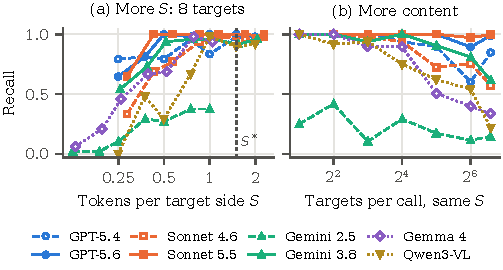
\includegraphics[width=\columnwidth]{figures/fig2.pdf}
\caption{Controlled images, eight models. (a) Recall rises gradually with $S$ (8 targets, 8 distractors); dashed line: $S^\ast = 1.5$. (b) At fixed $S$ (1.25 to 1.43 for resolution-scaled models), recall falls as a call must report more targets; lowest reasoning setting, Sonnet 5.5 with adaptive thinking. Dashed and hollow: older generation. $1024^2$ canvas, six images per point; mean matched recall per image; no intervals shown. The fixed-grid models in (b) have $S$ of 0.63 to 1.29.}
\label{fig:curves}
\end{figure}

\subsection{\texorpdfstring{Cause two: $L$}{Cause two: L}}

Adding content to a call while $S$ stays fixed lowers recall. On controlled images with the canvas, $S$ and tokens fixed, Qwen3-VL recalls \XcapNlastqwenThreevl{} of 96 targets, against \XcapNtwoqwenThreevl{} of two (\cref{fig:curves}b). On drawing sheets, packing eight tiles into one GPT-5.6 call at the same tokens per target lowers recall from \XmosRgptFiveSixkOne{} to \XmosRgptFiveSixkEight{} (difference \XmosdRgptFiveSixkEight, 95\% interval \XmosdRCIgptFiveSixkEight), although a packed call must report a median of only \CpackMedian{} targets (mean \CpackMean, at most \CpackMax). The failures occur in answers that end normally: in the controlled sweep \CcapNormal{} of \CcapCalls{} calls ended normally (the other is a Gemini 3.8 call whose thinking used the output cap), and the longest visible answer used \CcapMaxOut{} of the 8{,}192 tokens allowed. Where recall starts to fall depends on the model, content and reasoning setting: on the controlled images Sonnet 4.6 and GPT-5.4 drop from about 32 targets and GPT-5.6 and Sonnet 5.5 hold to 96, yet GPT-5.6 drops on packed drawing tiles. Lowering $L$ helps only where $L$ binds; splitting without enlarging does not help when $S$ is too small, and in the zoom-agent ablation (\cref{sec:agents}) lowering $L$ alone gave no significant gain, while enlarging gave GPT-5.6 \UnHThreegptFiveSixOVZOVC{} F1.

Part of the content limit holds for every model. Reporting $n$ positions in an area $A$ to within $\tau$ needs information:

\begin{theorem}[What a hit costs]
\label{thm:capacity}
For $n$ target centres independent and uniform on a region of area $A$ and any returned set $\hat Y$, $\mathbb{E}[\mathrm{Rec}] \cdot \Lbit \le I(Y; \hat Y) + o$, with $\mathrm{Rec}$ the matched recall and $\Lbit = n \log_2\!\big(A/(n\pi\tau^2)\big)$, where $o$ charges unmatched returned points and is $\log_2(n+1)$ without them.
\end{theorem}

Each hit therefore costs about $\log_2$ of the ratio between the area per target and the tolerance disk, in bits, so an answer that carries $C$ bits about positions can find at most about $(C + o)/\Lbit$ of the targets.


\subsection{What better models change, and why splitting stays}

\emph{The $S$ a model needs falls with each generation.} On the same token grid and the same controlled images, Gemini 3.8 recalls \UtOneHThree{} more than Gemini 2.5; and Gemini 4 receives the same 1{,}090 tokens per image as Gemini 3.8, yet the $S$ it needs for recall and precision of 0.9 falls from \CgenSninetyGemThreeEight{} to \CgenSninetyGemFour{} (both at the vendor's default reasoning; \supp{D}). On this grid the whole image already reaches that $S$ on \CreachGemThreeEight{} of the \CreachN{} LegendSpot drawings for Gemini 3.8 and on \CreachGemFour{} for Gemini 4, so fewer images need splitting.
\emph{What one call can handle grows.} With 96 targets on the same controlled images, recall rises from \XcapNlastgptFiveFour{} (GPT-5.4) to \XcapNlastgptFiveSix{} (GPT-5.6) and from \XcapNlastsonnetFourSix{} (Sonnet 4.6) to \XcapNlastsonnetFiveFive{} (Sonnet 5.5, with adaptive thinking); in our sweep of targets per call at $S = 1.5$, GPT-6.1 holds at \CgenGptSixOneMax{} targets (\cref{tab:thumb}, \supp{L}).
\emph{But the need to split stays.} An image can be arbitrarily large while a call's budget is fixed, and at the $S$ a model needs one call sees only a bounded area (\cref{prop:geometry}): each generation raises how much one call can handle, but no model removes the need to split.

The minimum cost also binds strategies that choose their own views. Let a call carry several images, as when an agent keeps earlier views, and count all their tokens.

\begin{proposition}[Recall-cost frontier]
\label{prop:frontier}
Suppose a policy sees the image only through the model's responses and makes a bounded number of calls, and that, given any history, adding one target changes the law of the model's response by at most $\sum_I f(S_I)$ in total variation, summed over the images $I$ of the call that show it at $S_I$, with $f$ non-decreasing (graded recognition). To find a target placed anywhere in a region $\Omega$ with average probability $\bar R$, the policy's expected tokens on images without that target are at least
\[
\frac{\bar R\,|\Omega| - \pi\tau^2\,\overline{\mathrm{FP}}_0}{\beta\,\kappa_f\, m^2}, \qquad \kappa_f = \sup_{S>0} f(S)/S^2,
\]
where $\overline{\mathrm{FP}}_0$ counts its false points there and $\beta \ge 1$ bounds $(1 + w/a_x)(1 + h/a_y)$ over its $a_x \times a_y$ views.
\end{proposition}

The bound covers policies that adapt, mix scales, randomize, or trade false points for hits, such as the zoom agents we test (\cref{sec:practice}). A high-resolution mode changes $S$ but not $L$, so it addresses at most the first cause.
